\chapter{基于神经网络的滑模控制方法研究}
\section{引言}很多的扰动补偿方法已经用于改善经典滑模控制方法,比如第三章提到的递推最小二乘法,还有干扰观测器以及神经网络补偿器等。其中,神经网络由于其不要求系统模型信息,在扰动补偿方面备受关注。但是在实际被控对象模型信息或者说扰动形式能够预先知道的情况下,加入特定的模型信息能够加快神经网络的收敛速度,进一步提高系统的扰动补偿能力。所以本节将精密直线运动平台系统特性引入到神经网络核函数的设计中,以提高系统的扰动补偿能力。

本章首先介绍了基于径向基函数(Radial Basis Function, RBF)神经网络的自适应补偿器设计,然后充分考虑精密直线运动平台的系统特性,提出了一种基于多核神经网络的动态边界层滑模控制方法,将精密直线运动平台定位力、摩擦力的经典模型考虑到神经网络核函数的设计中,进一步提高系统的位置跟踪性能和扰动抑制能力。
\begin{comment}
%\section{滑模控制基本原理}
考虑单输入动态系统\cite{slotine2006应用非线性控制}
\begin{equation}
\label{4单输入动态系统}
x^{(n)}=f(\textbf{x})+b(\textbf{x})u
\end{equation}
式中,标量$x$是控制系统输出(如精密直线运动平台的位置),标量$u$是控制信号输入(比如电机的出力),向量$\textbf{x}=[x,\dot{x},\dots,x^{n-1}]^T$为状态向量。$f(\textbf{x})$通常表示一个非线性函数,用来表示系统的扰动,虽然不能精确知道,但一般都认为它的上界是$\textbf{x}$的连续函数。$b(\textbf{x})$也认为不能精确已知,但是其不确定性也认为是有界的,比如PMLSMs模型参数慑动等。

为了使有限控制$u$实现跟踪任务,期望状态的初始值$\textbf{x}_d(0)$必须满足
\begin{equation}
\label{初态}
\textbf{x}_d(0)=\textbf{x}(0)
\end{equation}
即当$t=0$时控制系统输出与目标轨迹一致,这一条件在实际精密运动控制中基本都会满足,因为系统的位置和速度不会突变。

记跟踪误差为$e=x_d-x$,则跟踪误差向量为 $\textbf{e}=\textbf{x}_d-\textbf{x}=[e \quad\dot {e} \quad\cdots \quad e^{n-1}]^T$。用标量方程$s(\textbf{e};t)=0$定义状态空间$R_n$中的时变曲面$S(t)$
\begin{equation}
\label{滑模面0}
	s(\textbf{e};t)=\left(\frac{\text{d}}{\text{dt}}+\lambda\right)^{n-1}e
\end{equation}
式中,$\lambda$为一正常数。$n$表示系统的阶数,比如机械系统,大部分会是二阶系统,即$n=2$,此时
\begin{equation}
\label{滑模面1}
s=\lambda e+\dot{e}
\end{equation}
即$s$仅是位置误差和速度误差的加权和。
给定初始状态(\ref{初态}),跟踪问题$\textbf{x}\equiv\textbf{x}_d$则等价于当$t$\textgreater$0$时,使状态轨线停留在曲面$S(t)$上。实际上$s\equiv0$代表一个线性微分方程,假定初始条件为式(\ref{初态}),则其唯一解为$\tilde{\textbf{x}}\equiv0$。因此,跟踪$n$维向量$\textbf{x}_d$的问题可简化为标量$s$恒为零的问题。

更进一步,通过选择式(\ref{4单输入动态系统})中的控制信号$u$,使得状态轨线在曲面$S(t)$之外满足下式
\begin{equation}
\label{收敛条件}
\frac{1}{2}\frac{\text{d}}{\text{dt}}s^2\leq-\eta\left|s\right|
\end{equation}
从而保证$s$恒为零的问题简化为一阶问题,其中$\eta$为正常数。本质上,式(\ref{收敛条件})表示的是以$s^2$为度量到曲面的平方``距"沿所有系统轨线减小,因此系统轨线就会不断趋向于曲线$S(t)$。如图\ref*{滑动条件}所示,轨线只要能够进入曲面就会一直停留在该曲面上。从另一个角度来说,系统轨线满足式(\ref{收敛条件}),就会使曲面成为一个不变集。满足式(\ref{收敛条件})的曲面$S(t)$称为滑动曲面,且当系统状态在曲面上时就被称为滑动模或滑动形态。

实际上,即使式(\ref*{初态})不满足,即初始时刻,系统输出与系统目标轨迹不一致,也就是说,系统不满足零状态,系统轨线仍然能够在小于$s(t=0)/\eta$的有限时间内到达曲面$S(t)$。总的来说,这种通过设计滑模面$S(t)$,并合理设计控制律$u$以使系统状态轨迹收敛到滑模面上的方法,成为滑模控制,是一种有效的容易实现的鲁棒控制方法。
\begin{figure}
	\centering
	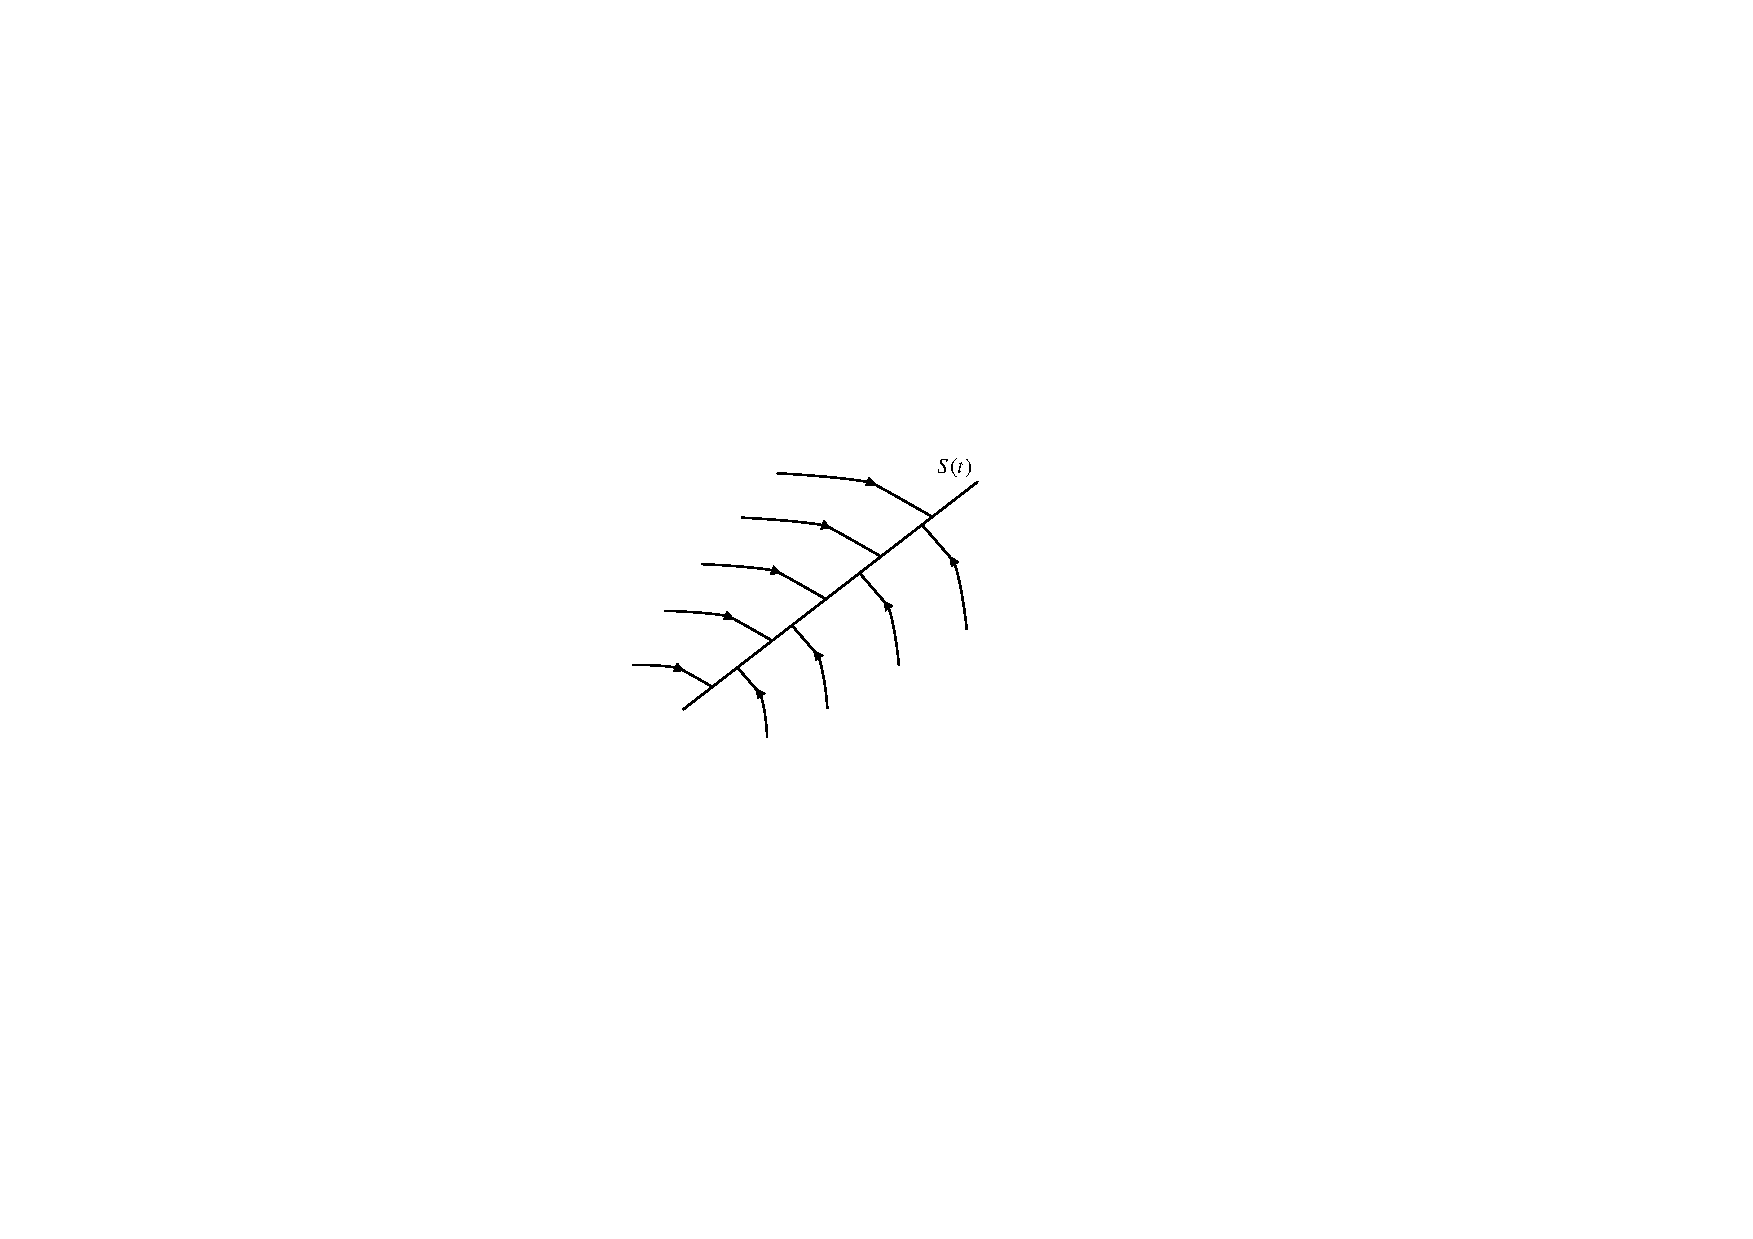
\includegraphics[width=10cm]{figures/滑动条件}
	\caption{滑动条件}
	\label{滑动条件}
\end{figure}
\end{comment}
%\section{基于传统RBF神经网络的滑模控制器设计}

\section{基于传统RBF神经网络的自适应补偿器设计}
%1985年,Powell提出了多变量插值的RBF方法。RBF是一个取值仅仅依赖于离原点距离的实值函数,也就是$\phi(x)=\phi(\norm{x})$,或者还可以理解为到任意一点$c$的距离,$c$点定义为中心点,也就是$\phi(x,c)=\phi(\norm{x-c})$。凡是满足$\phi(x)=\phi(\norm{x})$性质的函数$\phi$都可以称为RBF。经典的RBF一般使用欧氏距离(也叫做欧式RBF),尽管其他距离函数也可以满足RBF的定义。
%最常用的RBF神经网络是基于高斯核函数建立的,形式为
%
%\begin{equation}
%k\left(\norm{x-x_c}\right)=\text{exp}\left(\frac{-\norm{x-x_c}^2}{(2\sigma)^2}\right)
%\end{equation}
%其中,

%$x_c$为核函数中心点,类似于输入信号的平均值;
%
%$\sigma$为函数的宽度参数,类似于输入信号的标准差,决定了函数的径向作用范围。

传统的RBF神经网络凭借对于非线性函数强大的拟合能力\cite{1987Powell},常被用来作为前馈补偿器在线补偿精密直线运动平台的集总扰动,然后通过一定的规则对其权重参数进行在线调整。这里选用网络结构为1-5-1,如图\ref{RBF网络结构}所示。其中,$h_i\,(i=1,2,3,4,5)$表示隐含层5个高斯核函数节点。
\\
\begin{figure}[H]
	\centering
	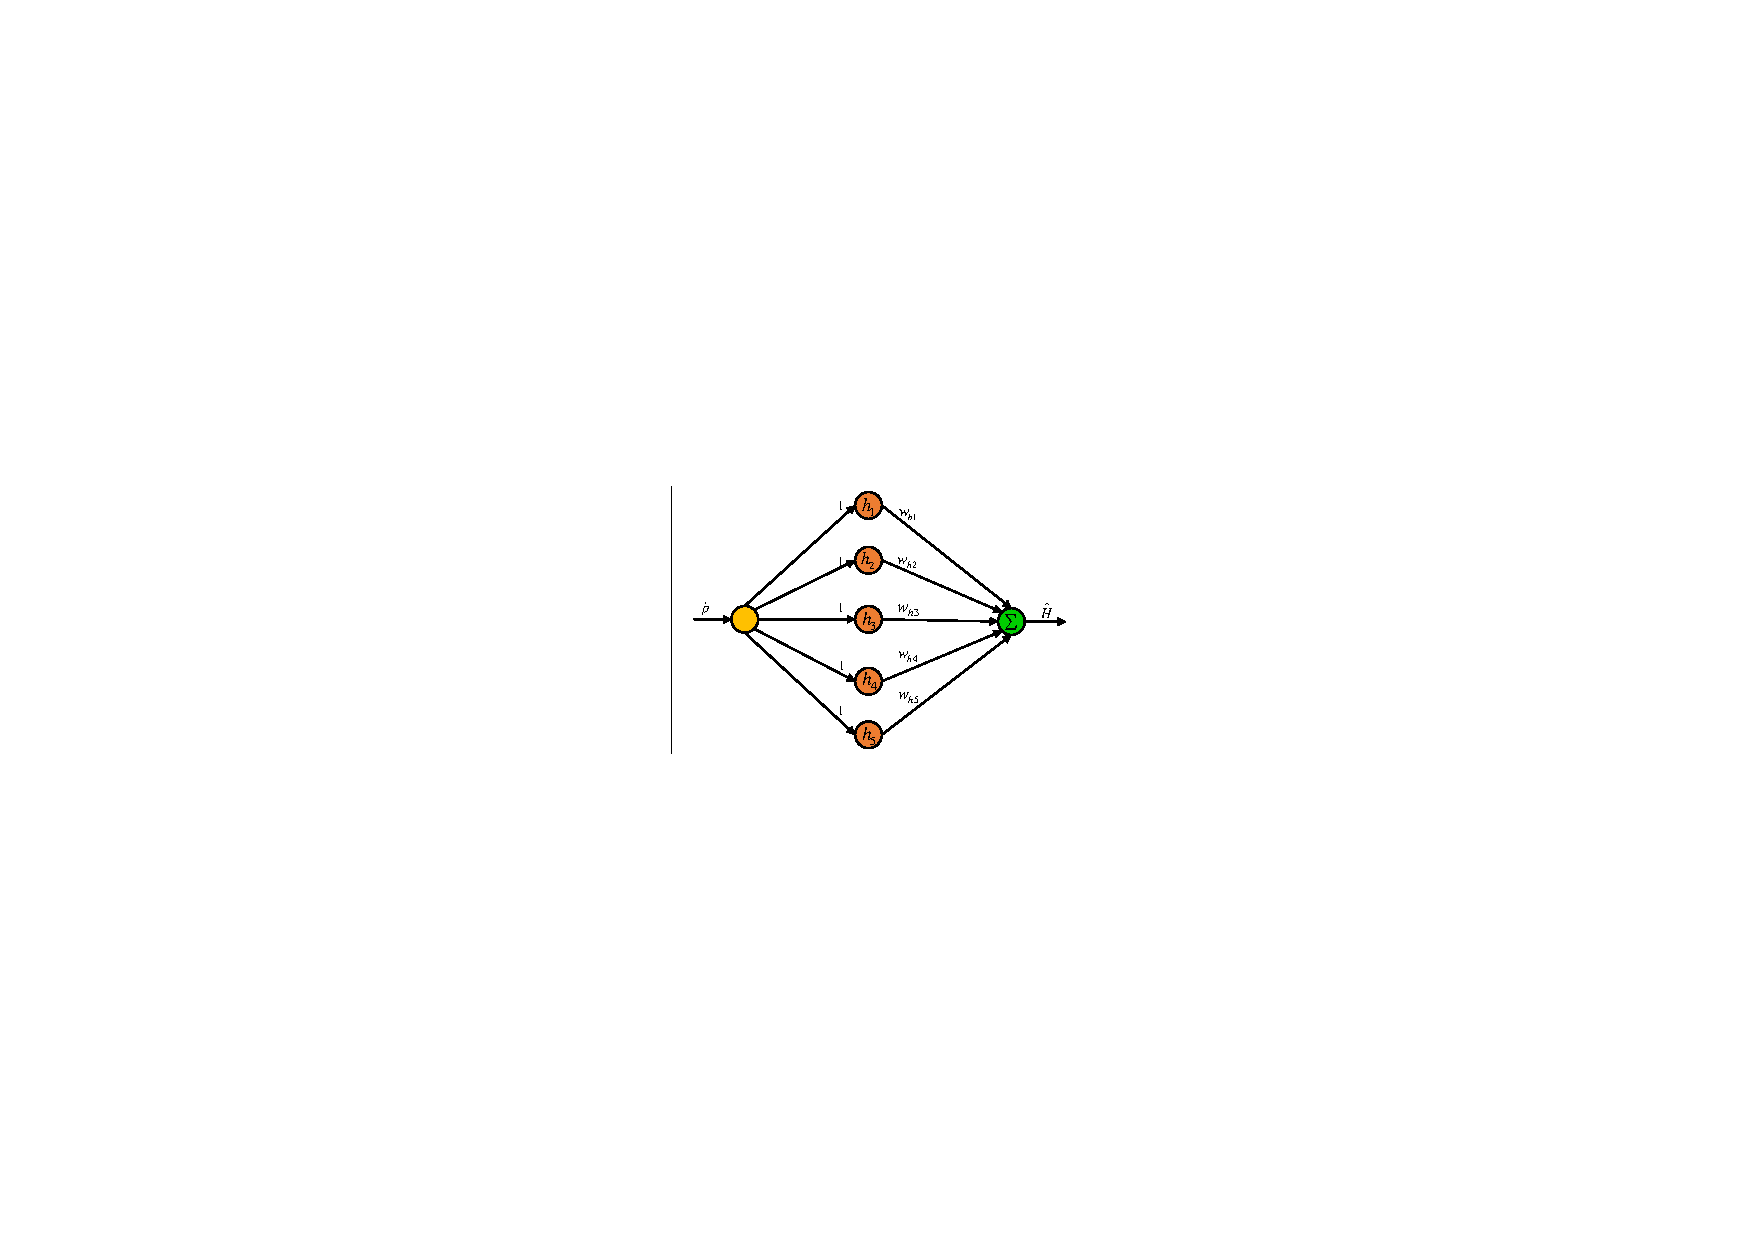
\includegraphics[width=12cm]{figures/RBF神经网络结构.pdf}
	\caption{RBF网络结构}
	\label{RBF网络结构}
\end{figure}

RBF神经网络的算法可以表示为
\begin{equation}
\begin{aligned}
&h_i=\text{exp}\left(\frac{-\norm{x_i-c_i}^2}{2{b_i}^2}\right)\\
&H(x)={\textbf{\textit{W}}^{*T}}h(x)+\varepsilon\\
\end{aligned}
\end{equation}
式中,

$x_i$为第$i$个隐含层的输入;

$c_i$为第$i$个隐含层核函数中心点,类似于输入信号的平均值;

$b_i$为第$i$个隐含层核函数的宽度参数,类似于输入信号的标准差,决定了函数的径向作用范围;

$h(x)$为隐含层的输出;

$\textbf{\textit{W}}^*$为隐含层到输出层的理想权重;

$\varepsilon$为神经网络的逼近误差,$\left|\varepsilon\right| <{{\varepsilon }_{max}}$。

传统的RBF神经网络的输入选为精密直线运动平台的速度信号$\dot{p}$,网络输出为对$H$的估计
\begin{equation}
\hat{H}={\hat{\textbf{\textit{W}}}}^{T}h(\dot{p})
\end{equation}
式中,$\hat{\textbf{\textit{W}}}$为隐含层到输出层的估计权重,取$\tilde{\textbf{\textit{W}}}=\hat{\textbf{\textit{W}}}-\textbf{\textit{W}}^*$,则有
\begin{equation}
H-\hat{H}=-{{\tilde{\textbf{\textit{W}}}}^{T}}h+\varepsilon
\end{equation}
表示传统RBF神经网络估计值与理想值之间的差别。在实际的精密直线运动平台中,用$\hat{H}$来实现对系统集总扰动的在线补偿,即实现了基于传统RBF神经网络的补偿器。在设计流程中,重要的是确定网络结构以及高斯核函数的参数,即核函数中心点和宽度参数,这里都根据经验选取,即中心点假设根据输入信号均匀分布进行确定,宽度参数假设相邻中心点的差值。

\section{基于多核神经网络的动态边界层滑模控制器设计}
为了实现PMLSM的高性能控制,本文提出了一种带有动态边界层的多核神经网络滑模控制(Multi-Kernel Neural Network Sliding Mode Control, MNNSMC)方法。该方法采用多核神经网络对系统非线性扰动进行在线补偿。其中,核函数的设计不仅基于传统的高斯核函数,还引入了三角核函数和sigmoid核函数,极大程度地抑制了PMLSM定位力、摩擦力等各种不确定因素带来的影响,提高了系统的跟踪性和鲁棒性。另一方面,采用边界层可动态调整的饱和函数,不仅可以削弱抖振,还可以保证系统状态轨迹渐近收敛到切换平面。基于MNNSMC的PMLSM运动控制系统的控制框图如图\ref{MNNSMC控制架构}所示,下面具体介绍各部分的设计。
\begin{figure}[H]
	\centering
	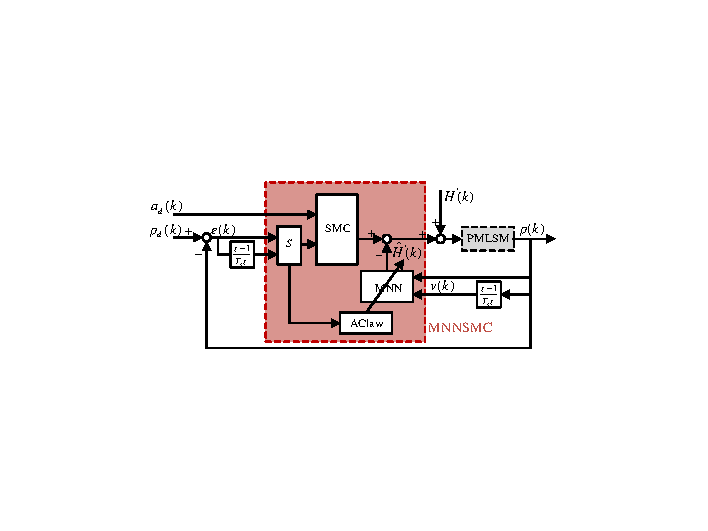
\includegraphics[width=12cm]{figures/MNNSMC控制架构1.pdf}
	\caption{基于MNNSMC的PMLSMs控制系统框图}
	\label{MNNSMC控制架构}
\end{figure}

\begin{comment}
与基于传统RBF神经网络的滑模控制设计不同的部分在于神经网络和边界层的设计部分,分别如4.4.1节和4.4.2节所述,神经网络部分相比于传统的基于单核(高斯核函数)的RBF神经网络改进为考虑了PMLSMs扰动模型结构的多核神经网络(MNN),边界层部分将经典的固定边界层饱和函数改进为动态边界层饱和函数(DBSMC),稳定性的证明和多核神经网络权重的自适应律都是基于Lyapunov理论得出,最终得到的改进的控制律为
\begin{equation}
\label{4-29}
\begin{aligned}
U& =\frac{1}{{{B}_{n}}}\left[\lambda \dot{e}+{{{\ddot{p}}}_{d}}-\hat{H^{'}}+\eta \text{sat}\left(\frac{S(t)}{\Delta(\dot{p})}\right)\right] \\ 
& ={{U}_{eq}^{'}}+{{U}_{nn}^{'}} \\ 
\end{aligned}
\end{equation}
其中,
\begin{equation}
\label{4-30}
\begin{aligned}
U_{e q}^{'}&=\frac{1}{B_{n}}\left[\lambda \dot{e}+\ddot{p}_{d}+\eta \operatorname{sat}\left(\frac{S(t)}{\Delta(\dot{p})}\right)\right] \\
U_{n n}^{'}&=-\frac{1}{B_{n}} \hat{H^{'}}
\end{aligned}
\end{equation}
式中,
%\text{sat}\left(\frac{S(t)}{\Delta(\dot{p})}\right)

$U_{eq}^{'}$为含动态边界层的滑模控制律;

$U_{nn}^{'}$为多核神经网络补偿律;

$\hat{H^{'}}$为多核神经网络的输出,这里将多核神经网络的隐含层输出统一表示为$h^{'}(x)$,则$\hat{H^{'}}(x)$为
\begin{equation}
\label{4-31}
\hat{H^{'}}(x)={\mathbf{W}^{T}}h^{'}(x)
\end{equation}

多核神经网络隐含层到输出层权重的更新律可以表示
\begin{equation}
\label{4-32}
\dot{\hat{\bf{W^{'}}}}=-{{\textbf{ }\!\!{\gamma}\!\!\text{}}^{-1}}Sh^{'}(x)\text{,}
\end{equation}
至此,多核神经网络滑模控制器方法设计完毕。
\end{comment}

\subsection{多核神经网络补偿器设计}
神经网络对于非线性函数有着良好的拟合能力,在扰动补偿方面很受欢迎\cite{zhao2019adaptive,sun2019adaptive}。但是传统的神经网络往往是一个“黑箱模型”,在处理集总扰动时没有充分利用系统扰动的特性。

正如第二章讨论的一样,PMLSMs系统的定位力和摩擦力是扰动的主要来源,而且有很多经典的模型已经被提出,专门用来近似定位力和摩擦力,因此对其进行辨识和补偿可以在一定程度上提高精密直线运动平台的扰动抑制能力。这里充分利用PMLSMs系统扰动的一些特性,将定位力与摩擦力的经典模型考虑到神经网络核函数的设计中,提出了一种多核神经网络(Multi-Kernel Neural Network, MNN)补偿器,其结构如图\ref*{MNN结构}所示。该结构中保留了RBF神经网络经典的3层结构。隐含层中不仅用经典的高斯核函数补偿时变的扰动,如图中$f_1$,还引入了三角核函数,以及sigmoid核函数,分别对应补偿定位力和摩擦力带来的扰动,如图中$f_2$。三种核函数的具体形式为:
\\
\begin{figure}[H]
	\centering
	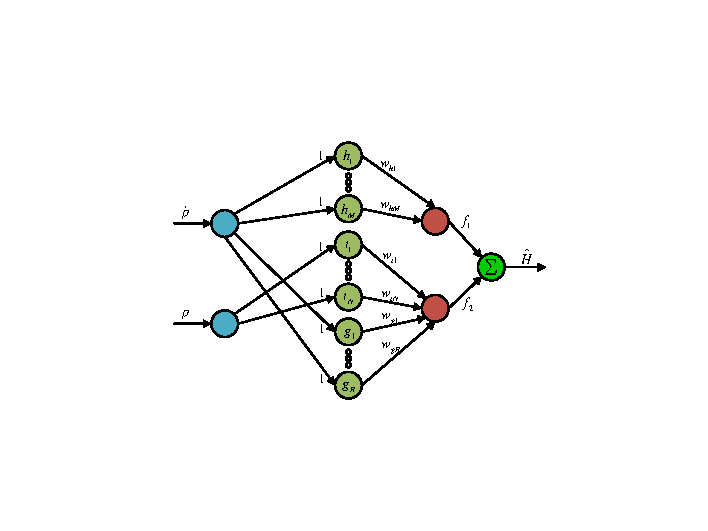
\includegraphics[width=12cm]{figures/MNN.pdf}
	\caption{多核神经网络结构}
	\label{MNN结构}
\end{figure}
\begin{enumerate}
	\item[A.] \textbf{高斯核函数}. 高斯核函数的数学描述为
	\begin{equation}
	{{h}_{j}}=\text{exp}(-\frac{{{({{x}_{j}}-{{c}_{j}})}^{2}}}{2b_{j}^{2}})
	\end{equation}
	式中,$h_j$为第$j$个高斯核函数的输出;$x_j$为第$j$个高斯核函数的输入;$c_j$,\,$b_j$分别为第$j$个高斯核函数的中心的宽度参数,统计学意义上分别相当于输入信号的均值和方差;$j$=1, 2, $\cdots$, $N_h$;$N_h$是高斯核函数的个数。
	\item[B.] \textbf{三角核函数}. 三角核函数的数学描述为
	\begin{equation}
	{{t}_{k}}=\left\{ \begin{aligned}
	&\text{sin}(\frac{2\text{ }\!\!\pi\!\!\text{ }{{n}_{k}}}{{{\tau }_{s}}}{{x}_{k}})\text{,} \\ 
	&\text{cos}(\frac{2\text{ }\!\!\pi\!\!\text{ }{{n}_{k}}}{{{\tau }_{s}}}{{x}_{k}})\text{,} \\ 
	\end{aligned} \right.
	\end{equation}
	式中,$t_k$是第$k$个三角核函数的输出;$x_k$是第$k$个三角核函数对的输入;$\tau_s$是PMLSMs定位力的基频所对应的空间周期;\,$n_k$是PMLSMs定位力的谐波次数,通常为1,2,4,6等;$k$=1, 2, $\cdots$, $N_t$;$N_t$是三角核函数对的个数。
	\item[C.]\textbf{sigmoid 核函数}. sigmoid核函数的数学描述为
	\begin{equation}
	{{g}_{r}}=\frac{1-\text{exp}(-{{x}_{r}})}{1+\text{exp}(-{{x}_{r}})}
	\end{equation}
	式中,$g_r$第$r$个sigmoid核函数的输出;$x_r$是第$r$个sigmoid核函数的输入; $r$=1, 2, $\cdots$, $N_r$;$N_r$是sigmoid核函数的个数。
\end{enumerate}

基于前文设计的多核神经网络结构,这里为了简化,将神经网络的输出统一表述为
\begin{equation}
H(x)={\textbf{\textit{W}}^{*T}}h(x)+\varepsilon
\end{equation}
式中,

$x$为各隐含层的输入;

$h(x)$为隐含层的输出;

$\textbf{\textit{W}}^*$为隐含层到输出层的理想权重。其中,$\varepsilon$为神经网络的逼近误差,$\left|\varepsilon\right|\le\varepsilon_{max}$。网络输出为对$H(x)$的估计
\begin{equation}
\hat{H}={\hat{\textbf{\textit{W}}}}^{T}h(x)
\end{equation}
式中,$\hat{\textbf{\textit{W}}}$为隐含层到输出层的估计权重,取$\tilde{\textbf{\textit{\textbf{\textit{W}}}}}=\hat{\textbf{\textit{W}}}-\textbf{\textit{W}}^*$,则有
\begin{equation}
H-\hat{H}=-{{\tilde{\bf{W}}}^{T}}h+\varepsilon
\end{equation}
\subsection{基于多核神经网络的滑模控制器设计}
如式(\ref{2.14})所示,PMLSMs系统模型为
\begin{equation}
\label{(4-10)}
\begin{aligned}
\ddot{p}&=({{A}_{n}}+\Delta A)U+L \\ 
&={A}_{n}U+H  
\end{aligned}
\end{equation}

定义系统位置跟踪误差为
\begin{equation}
\label{4-11}
e=p_d-p
\end{equation}
两边对时间求导,可以得到误差对时间的导数为
\begin{equation}
\label{4-12}
\dot{e}=\dot{p_d}-\dot{p}
\end{equation}
滑模控制部分的设计主要包括两部分:滑模面的设计和控制律的设计。
这里设计滑模面为
\begin{equation}
\label{4-13}
S=\lambda e+\dot{e}
\end{equation}
式中,$\lambda$为一正常数。

根据式(\ref{(4-10)})和(\ref{4-12}),可以得出滑模面对时间的一阶导数为
\begin{equation}
\label{4-14}
\begin{aligned}
\dot{S}&=\lambda \dot{e}+\ddot{e} \\ 
&=\lambda\dot{e}+{{{\ddot{p}}}_{d}}-\ddot{p} \\ 
&=\lambda \dot{e}+{{{\ddot{p}}}_{d}}-{{A}_{n}}U-H  
\end{aligned}
\end{equation}
这里考虑到系统状态轨线的初始状态可能与目标轨迹的初始状态不一致,即系统可能不是零状态,因此需要一定的到达阶段才能保证系统进入滑动模态,同样,这里选定到达阶段的趋近律为等速趋近律
\begin{equation}
\dot{S}=-\eta\text{sgn}(S)
\end{equation}
式中,
%$\text{sgn}(\cdot)$为符号函数;
$\eta$为正常数,与神经网络逼近误差之间满足$\eta\ge\left|\varepsilon_{max}\right|$,主要决定到达阶段的趋近速率。

根据(\ref{4-13})和(\ref{4-14}),可以得出基于多核神经网络的滑模控制器的控制律为
\begin{equation}
\label{4-16}
\begin{aligned}
U& =\frac{1}{{{B}_{n}}}[\lambda \dot{e}+{{{\ddot{p}}}_{d}}-\hat{H}+\eta \text{sgn} (S)] \\ 
& ={{U}_{eq}}+{{U}_{nn}} \\ 
\end{aligned}
\end{equation}
其中,
\begin{equation}
\label{4-17}
\begin{aligned}
U_{e q}&=\frac{1}{B_{n}}\left[\lambda \dot{e}+\ddot{p}_{d}+\eta \operatorname{sgn}(S)\right] \\
U_{n n}&=-\frac{1}{B_{n}} \hat{H}
\end{aligned}
\end{equation}
式中,
$U_{eq}$为滑模控制律;$U_{nn}$为神经网络补偿律。

为了证明整个控制系统的稳定性,同时获得多核神经网络隐含层到输出层的权重更新律,选择Lyapunov函数为
\begin{equation}
\label{4-18}
V=\frac{1}{2}{{S}^{2}}+\frac{1}{2}{{\tilde{\textbf{\textit{W}}}}^{T}}\symbf{\gamma}\tilde{\textbf{\textit{W}}}
\end{equation}
式中,$\symbf{\gamma}$为一对角阵,且元素均大于0。两边对时间求导,可得
\begin{equation}
\label{4-19}
\dot{V}=S \dot{S}+\tilde{\textbf{\textit{W}}}^{T}\symbf{\gamma} \dot{\tilde{\textbf{\textit{W}}}}
\end{equation}
结合式(4.9)、式(\ref{4-14})、式(\ref{4-16})、式(\ref{4-17})和式(\ref{4-19}),
\begin{equation}
\label{4-20}
\begin{aligned}
\dot{V}&=-\eta S\text{sgn}(S)+S{{{\tilde{\textbf{\textit{W}}}}}^{T}}h(x)-S\varepsilon +{{{\tilde{\textbf{\textit{W}}}}}^{T}}\symbf{\gamma}\dot{\hat{\textbf{\textit{W}}}} \\ 
&=-\eta S\text{sgn}(S)-S\varepsilon +{{{\tilde{\textbf{\textit{W}}}}}^{T}}(Sh(x)+\symbf{\gamma}\dot{\hat{\textbf{\textit{W}}}}) \\ 
&=-\eta \left| S \right|-S\varepsilon +{{{\tilde{\textbf{\textit{W}}}}}^{T}}(Sh(x)+\symbf{\gamma}\dot{\hat{\textbf{\textit{W}}}})\text{.} \\ 
\end{aligned}
\end{equation}
取自适应律为 
\begin{equation}
\label{4-21}
\dot{\hat{\textbf{\textit{W}}}}=-\symbf{\gamma}^{-1}Sh\text{,}
\end{equation}
将自适应律代入式(\ref{4-20}),可以得到
\begin{equation}
\label{4-22}
\dot{V}=-\eta\left|S\right|-S\varepsilon\le 0\text{.}
\end{equation}
式(\ref{4-22})中,取$\dot{V}\equiv0$,则$S\equiv0$,由LaSalle不变集定理可知,当$t\to\infty,S\to0$。因此,多核神经网络滑模控制器的渐近稳定性得以证明。

式(\ref{4-17})中的滑模控制律之所以有较强的鲁棒性,主要在于有切换功能的开关函数,但开关函数会引起控制信号较大的抖振,往往用原点附近连续的饱和函数替代原点附近不连续的开关函数以削弱抖振,传统的固定边界层饱和函数可表示为
\begin{equation}
\label{4-23}
\operatorname{sat}\left(\frac{S}{\Delta}\right)=\left\{\begin{array}{ll}
1 & \mathrm{~S} \geq \Delta \\
\frac{S}{\Delta} & -\Delta<S<\Delta \\
-1 & \mathrm{~S} \leq-\Delta
\end{array}\right.
\end{equation}
式中,$\Delta$为边界层厚度,其取值往往依靠经验选取,选取的值过大,可以削弱抖振,但同时会造成稳态误差,进而对位置跟踪精度产生影响;取值过小,则对于削弱抖振效果不明显\cite{jin2007investigation}。固定边界层如图\ref{固定边界层}所示,其中,$\Delta$为边界层宽度。从图\ref{固定边界层}中可知,切换平面$S=0$位于边界层中间,在边界层内部相当于线性控制,因此无法保证系统在边界层厚度内稳定,即$[-\Delta,\Delta]$区间内保证稳定,这就使得系统在边界层内不能快速的响应外界扰动,降低了鲁棒性,同时位置跟踪精度也无法保证渐近收敛到$0$。因此,设计新型的饱和函数,即能够保证系统状态轨迹渐近收敛到切换平面上的饱和函数有重要意义。具体的工作将在4.3.3节进行详细介绍。
\begin{figure}[H]
	\centering
	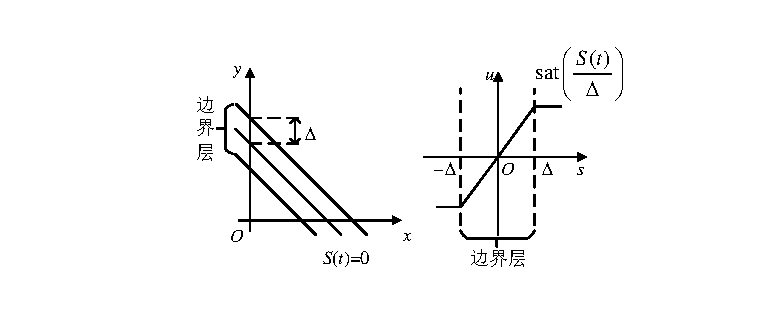
\includegraphics[width=12cm]{figures/固定边界层1.pdf}
	\caption{固定边界层}
	\label{固定边界层}
\end{figure}





\subsection{动态边界层设计}
如4.3.2节所述,设计新型饱和函数能够保证系统状态轨线渐近收敛到0,对于进一步提高PMLSMs系统位置跟踪精度具有重要意义。为了实现这一目的,边界层厚度随着系统状态轨迹变化而变化的饱和函数应运而生\cite{jin2007investigation},这里基于被控对象的系统特性,定义新型饱和函数为
\begin{equation}
\text{sat}\left(\frac{S(t)}{\Delta(\dot{p})}\right)=\left\{\begin{aligned}
&\frac{S(t)}{\Delta(\dot{p})} \quad&\left|\frac{S(t)}{\Delta(\dot{p})}\right|\le1\text{,} \\ 
&\text{sat}\left(\frac{S(t)}{\Delta(\dot{p})}\right) \quad&\left|\frac{S(t)}{\Delta(\dot{p})} \right|>1\text{,} \\ 
\end{aligned}\right.
\end{equation}
式中,$\Delta(\dot{p})$动态边界层厚度,考虑到PMLSMs系统位置跟踪误差与运动轨迹相关,在加减速段跟踪误差往往更大,需要更大的边界层厚度削弱抖振,匀速段跟踪误差相对较小。当系统状态轨迹到达边界层内部后,缩小边界层厚度可以保证系统状态轨迹渐近收敛到切换平面,进而保证位置跟踪误差渐近收敛到0。因此,本文将边界层厚度表示为系统输出速度的函数 
\begin{equation}
\Delta(\dot{p})={{\Delta}_{0}}(1-\alpha\left|{\dot{p}}\right|)
\end{equation}
式中,

$\Delta_0$为边界层厚度的初始值,即系统输出速度为0时的边界层厚度;

$\alpha$定义为边界层调节因子,为一非负常数。当系统到达边界层内时, $\Delta(\dot{p})$会逐渐减小,不断趋近于切换平面$S(t)$\,=\,0, $S(t)/\Delta(\dot{p})$的斜率会增加。当$\Delta(\dot{p})$\,$\to$\,0,$S(t)/\Delta(\dot{p})$的斜率无限增大,则新型饱和函数最终可以等效地看成开关函数 $\text{sgn}(\cdot)$,如图\ref{动态边界层}所示。因此,带有动态边界层的饱和函数即能够保证系统的快速切换,又能够保证原点附近的连续性,对削弱系统抖振和提高系统跟踪精度很有帮助。 
\begin{figure}[H]
	\centering
	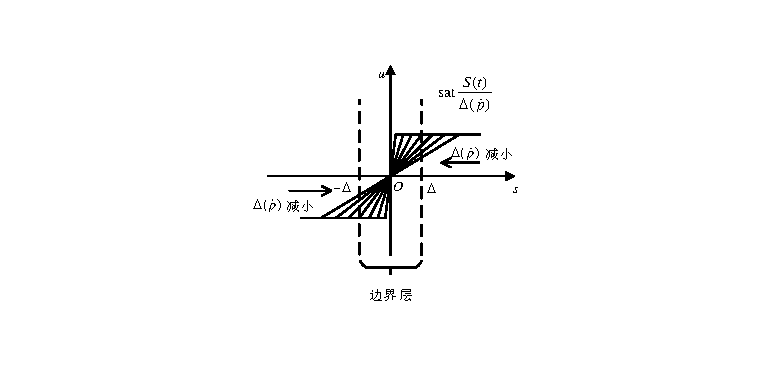
\includegraphics[width=12cm]{figures/动态边界层1.pdf}
	\caption{动态边界层}
	\label{动态边界层}
\end{figure}

\section{本章小结}
本章针对神经网络在滑模控制器设计中的应用进行了深入研究,介绍了基于传统RBF神经网络的自适应补偿器,提出了一种新型的带有动态边界层的MNNSMC方法。该方法包含MNN和滑模控制两个部分,其中,MNN将PMLSMs扰动的经典模型结构考虑到神经网络核函数的设计中,分别用三角核函数和sigmoid核函数补偿定位力和摩擦力等时不变的扰动,同时保留传统RBF的高斯核函数补偿时变的非线性扰。另一方面,提出了一种动态边界层饱和函数以进一步提高系统的位置跟踪能力。最后,通过构建关于滑模变量与神经网络权重的李雅普诺夫函数,证明了带有动态边界层的MNNSMC的渐近稳定性,从理论上表明了所提方法对于提高精密直线运动平台位置跟踪性能和扰动抑制能力的有效性。
%\newpage
%\mbox{}
%\newpage